\makeatletter\def\input@path{{../shared/}{../diagrams/}}\makeatother
\documentclass[11pt,a4paper]{article}
\usepackage{spirdoc}
\graphicspath{{img/}}
\SetDoc{SPIR-UG-001}{User Guide}{1.0}{Issued for review}
\Revisions{%
  1.0 & 27 Nov 2026 & \SPIRAuthor & First issue for release \SPIRRelease: supplier portal, company portal, phone scanning.\\
}
\newcommand{\shot}[3][0.92]{\begin{figure}[H]\centering\fcolorbox{spirrule}{white}{\includegraphics[width=#1\linewidth]{#2}}\caption{#3}\end{figure}}
\newcommand{\step}[1]{\item #1}

\begin{document}
\MakeCover{How to use SPIR day to day: suppliers entering shipments and printing QR labels, receiving staff scanning and checking parts.}
\DocumentControl
\tableofcontents
\clearpage

\section{Getting started}
SPIR has two portals and a public scan page. Open them in a browser; nothing needs installing.

{\small\zebra
\begin{tabularx}{\linewidth}{@{}L{3.2cm}L{5.4cm}Y@{}}
  \thead\hd{Who} & \hd{Address} & \hd{Sign-in}\\
  Suppliers & \textit{<SPIR address>}\code{/\#/supplier} & Username \code{admin}, password \code{admin}\\
  Receiving / quality & \textit{<SPIR address>}\code{/\#/company} & Username \code{admin}, password \code{admin}\\
  Anyone with a phone & Scan the QR label & No sign-in\\
\end{tabularx}}

\begin{caution}[Proof-of-concept sign-in]
The \code{admin} / \code{admin} sign-in is the same for everyone and will be replaced by personal accounts. Do not
enter real data on a public address until then.
\end{caution}

\shot[0.7]{sign-in}{Sign-in page (supplier portal). The company portal looks the same.}
If you see ``Wrong username or password'', check both fields and try again. Your session lasts 12 hours; sign out with
\ui{Sign out} at the top right. You can be signed in to both portals in the same browser at once.

% =====================================================================================
\section{Supplier portal}
\Diagram[0.55]{workflow-supplier}{The supplier's workflow.}

\subsection{Set up your profile (first time only)}
\begin{enumerate}
  \step{Sign in to the supplier portal and open \ui{Profile}.}
  \step{Enter your \ui{Supplier name} exactly as on your shipping labels. Country (2-letter code such as \code{IN}),
    contact person, e-mail, phone and address are optional.}
  \step{Click \ui{Save and continue}.}
\end{enumerate}
Every shipment and QR label you create carries this name. You can change it later; the change applies to all your
shipments.
\shot{supplier-profile}{Supplier profile.}

\subsection{The overview}
After the profile is set, \ui{Overview} shows the three steps (add data, print labels, keep it up to date) and counts of
your shipments, active QR labels and parts.
\shot{supplier-overview}{Supplier overview.}

\subsection{Add one shipment}
A shipment is \textbf{one part against one PO line}.
\begin{enumerate}
  \step{Click \ui{Add a shipment}.}
  \step{Fill in the fields marked \ui{required}: part number, part description, PO number, PO line, quantity, heat
    numbers and pattern number. Separate several heat numbers with commas.}
  \step{Optional: design revision, material, your own part number, country of origin, RT number.}
  \step{Click \ui{Save and create QR code}.}
\end{enumerate}
If something is wrong, the field is outlined in red with the reason underneath (for example ``Quantity must be a whole
number''). Fix it and save again.
\shot{shipment-form}{Shipment form with a field error.}

\paragraph{After saving} The shipment page opens with a green confirmation. From here you print the QR label (\ui{Show printable label}, then \ui{Print label}),
upload certificates and see the version history.
\shot{shipment-page}{Shipment page: hang tag, details, certificates, QR label and history.}

\subsection{Upload many shipments from a CSV file}
\begin{enumerate}
  \step{Open \ui{Upload CSV} and click \ui{Download a template}.}
  \step{Fill one row per shipment in Excel or another spreadsheet; save as CSV.}
  \step{Drop the file on the page or choose it, then click \ui{Import and create QR codes}.}
\end{enumerate}
If any row has a problem, \textbf{nothing is imported} and every problem is listed with its row number. Fix the file and
upload it again. Uploading an updated file later changes the data behind the same QR codes.
\shot{csv-upload}{CSV upload with the column guide.}

\begin{keypoint}[CSV columns]
\code{part\_number}, \code{part\_description}, \code{purchase\_order\_number}, \code{po\_line\_number}, \code{quantity},
\code{heat\_numbers} (several separated by \code{|}), \code{pattern\_number} are required. Optional: \code{design\_revision},
\code{material}, \code{radiographic\_test\_number}, \code{country\_of\_origin}. You do not need a supplier column: your
profile name is used.
\end{keypoint}

\subsection{Change a shipment}
Open the shipment (\ui{Shipments}, then the record ID) and click \ui{Edit shipment}. Change what you need and click
\ui{Save changes}. SPIR saves a new version; it is live immediately and the printed QR label shows the new data. Part
number, PO number and PO line cannot change because they identify the shipment. If one of them is wrong, add a new
shipment and revoke the old label.
\shot{shipments}{Your shipments, with version and QR status.}

\subsection{Upload certificates}
On the shipment page, under \ui{Certificates}, choose the document type (MTC, CoC, RT report, inspection report,
drawing, other), choose the file (PDF, PNG or JPEG, up to 15\,MB) and click \ui{Upload}. Uploads never replace earlier
files. Anyone who scans the label can open them.

\subsection{Print QR labels}
\begin{enumerate}
  \step{Open \ui{QR labels}. Each shipment's code is checked automatically (``Scan check passed'').}
  \step{Choose your sticker sheet: \ui{8}, \ui{14} or \ui{21 per sheet} (A4, Avery L7165, L7163, L7160 sizes).}
  \step{Tick the labels to print, or use the filter. To finish a part-used sheet, set \ui{Start at label}.}
  \step{Click \ui{Print \ldots{} labels}. In the print dialog choose A4, scale 100\,\% (\emph{Actual size}) and margins \emph{None}.}
\end{enumerate}
\shot{qr-labels}{QR labels: sheet layout, scan check and preview.}
\paragraph{Tips} If labels print slightly off, open \ui{Printer alignment}, print one page on plain paper with
\ui{Print label outlines} ticked, hold it against a sticker sheet and nudge in millimetres. \ui{Download PNGs} gives
one 300\,dpi image per label for label software. \ui{Export links as CSV} lists every label's link.

\subsection{Replace or revoke a label}
On the shipment page: \ui{Replace label} issues a new code (print it; the old label stops working);
\ui{Revoke label} stops the label without a replacement. A scan of a stopped label says it was revoked.

% =====================================================================================
\section{Company portal}
\Diagram[0.55]{workflow-receiving}{Receiving workflow.}

\subsection{Scan a QR code}
The company portal opens on \ui{Scan a QR code}.
\begin{itemize}
  \item \ui{Start camera}: point at the label; the shipment opens when the code is read.
  \item A USB or Bluetooth barcode scanner works too: click the page and scan.
  \item No camera: use \ui{Or paste the QR link or token}.
\end{itemize}
\shot{company-scan}{Scanner page.}
\shot{company-scanned}{A scanned shipment inside the company portal.}

\subsection{Search shipments}
\ui{Search shipments} lists every supplier's shipments. Type a PO number, part number, heat number or record ID.
\shot{company-search}{Search by heat number.}

\subsection{Check a product label}
Use this to compare the supplier's own sticker with what SPIR holds.
\begin{enumerate}
  \step{Open \ui{Check a product label} (or \ui{Check the sticker on this item} from a scanned shipment).}
  \step{Click \ui{Start camera} and \ui{Capture photo}, or \ui{Upload photo}. Hold the phone straight, avoid glare, and fill the frame with the label.}
  \step{Drag a box around the label text (crop) and click \ui{Read the label}.}
  \step{SPIR finds the shipment and shows every field: approved value, what was read, and the result.}
  \step{For any field marked for review, choose \ui{The reading is right}, \ui{Correct the reading} or \ui{Raise a discrepancy} and click \ui{Save review}. Then click \ui{Finalise check}; a finalised check can no longer be changed.}
\end{enumerate}
\shot{label-check}{Label check.}

{\small\zebra
\begin{tabularx}{\linewidth}{@{}L{3.4cm}Y@{}}
  \thead\hd{Overall result} & \hd{What to do}\\
  PASS & The label agrees with SPIR. Accept.\\
  PASS\_WITH\_\allowbreak WARNINGS & Agrees, but something optional was missing or uncertain. Accept after a glance.\\
  NEEDS\_REVIEW & SPIR is not sure (low confidence, possible misread). Check the marked fields by eye and confirm or correct.\\
  FAIL & A critical field differs (for example heat or quantity). Hold the part and record a discrepancy.\\
  UNRESOLVED & SPIR could not find the shipment. Retake the photo, crop tighter, or choose the record.\\
\end{tabularx}}

Label checks never change shipment data; they are kept as evidence in \ui{Label check history}.

% =====================================================================================
\section{Scanning with a phone (anyone)}
Open the phone's normal camera app and point it at the QR label; tap the link that appears. The page shows the
shipment (part, PO and line, quantity, heats, pattern, supplier) and a large button for each certificate. No sign-in
is needed.

\begin{figure}[H]\centering
\fcolorbox{spirrule}{white}{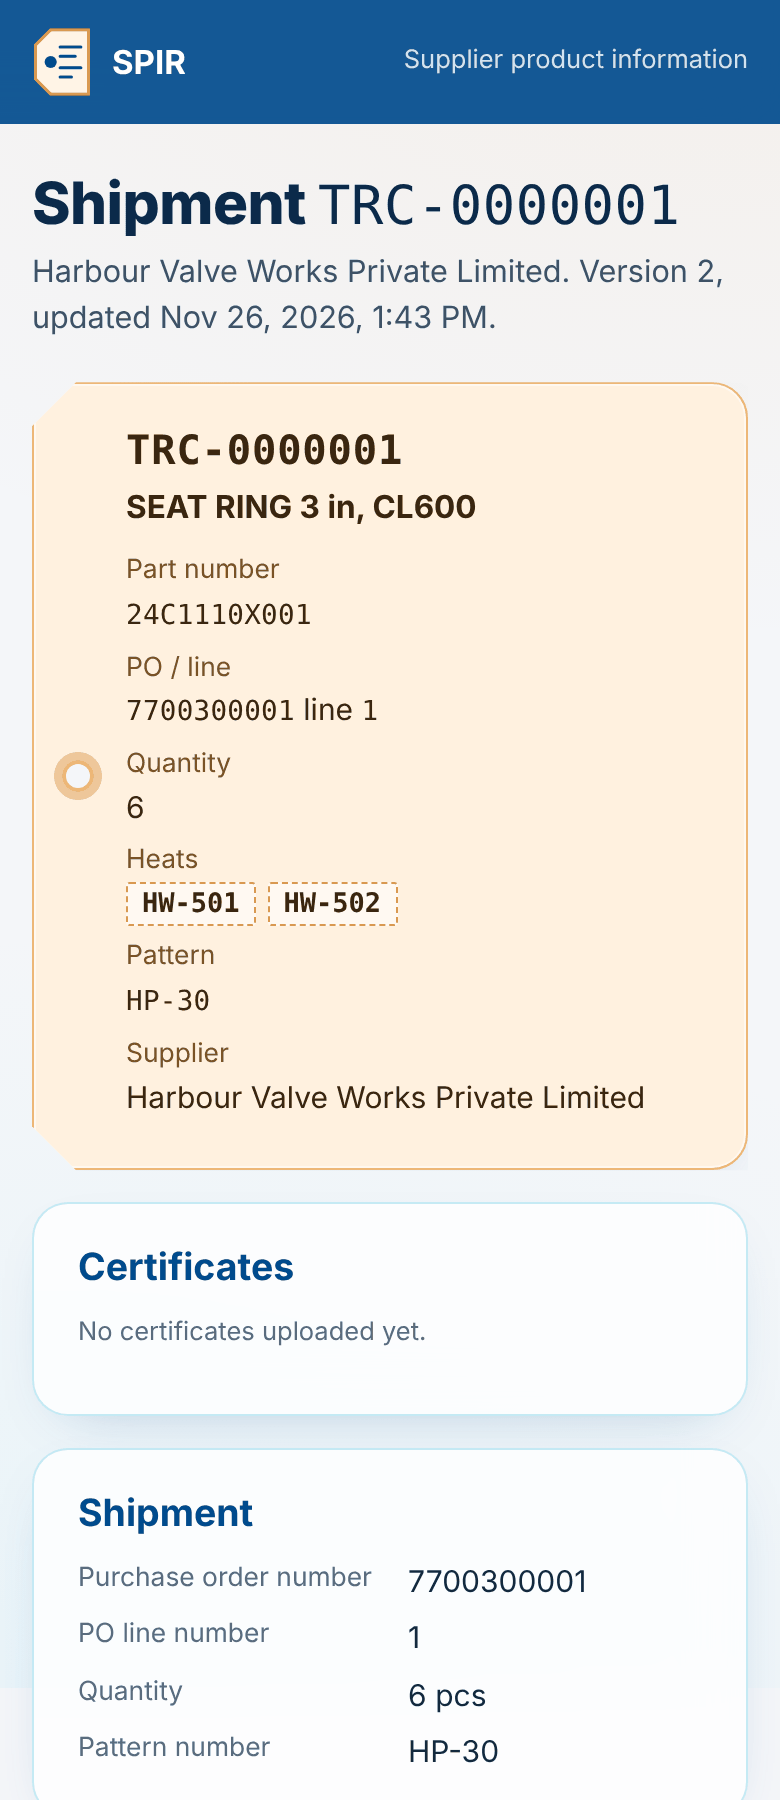
\includegraphics[width=0.36\linewidth]{public-scan}}
\caption{Public scan page on a phone.}
\end{figure}

\begin{itemize}
  \item ``This QR label has been revoked'': set the part aside and ask the supplier for a new label.
  \item ``SPIR doesn't recognise this QR label'': the label is damaged or not a SPIR label.
  \item The phone asks for a GitHub sign-in: the label was printed with a temporary development address. Ask for a
    reprint after the permanent address is set.
\end{itemize}

% =====================================================================================
\section{Frequently asked questions}
\begin{description}
  \item[Can I delete a shipment?] No. For traceability, shipments are never deleted; correct them with a new version or
    revoke the label.
  \item[Does editing break printed labels?] No. A label always shows the latest version.
  \item[Why can't I change the PO line?] Part number, PO and line identify the shipment and its QR code.
  \item[Who sees my data?] The company portal sees all suppliers' shipments; anyone who scans a label sees that one
    shipment and its certificates.
  \item[The camera does not start.] Allow camera access in the browser and use the HTTPS address.
\end{description}
\end{document}
